% compile with XeLaTeX or LuaLaTeX
\documentclass[10pt,a5paper,twoside]{article}
\usepackage{iftex}
\RequireXeTeX
\usepackage[top=12mm,bottom=26mm,outer=28mm,inner=14mm,foot=14mm]{geometry}
\usepackage{calc}
\usepackage{scrextend}
\deffootnote[1.5em]{0em}{1em}{\thefootnotemark\quad}
\renewcommand{\footnoterule}{%
  \kern -2.4pt
  \hrule width \textwidth height 0.4pt
  \kern 2pt
}

\usepackage{fontspec}
\setmainfont[
	Ligatures=TeX,
	Extension=.otf,
	SlantedFont=cmunsl,
	BoldFont=cmunbx,
	ItalicFont=cmunti,
	BoldItalicFont=cmunbi,
	SmallCapsFont=cmunrm, % for upright instead of slanted small caps
	SmallCapsFeatures={Letters=SmallCaps,Numbers=OldStyle},	
]{cmunrm}

\usepackage{etoolbox}
\usepackage{microtype,ellipsis}

\usepackage{polyglossia,iflang}
\setotherlanguage{russian} % the name of the original Russian version at the end of this book is written using Cyrillic letters

\usepackage{textcomp}

\usepackage{amsmath,amssymb,nicefrac,amscd}
\usepackage{graphicx,float}
\usepackage{import}
\usepackage{pdfpages}

\usepackage{enumitem}
\setitemize[1]{noitemsep,nosep,leftmargin=0.99em,label={--}}

\usepackage{transparent}
\usepackage{csquotes}
\DeclareQuoteStyle{vietnamese}
  {\textquotedblleft}
  {\textquotedblright}
  [0.05em]
  {\textquoteleft}
  {\textquoteright}

\usepackage{siunitx}
\sisetup{per-mode=fraction,fraction-function=\nicefrac}

\usepackage{hyperref}

\usepackage{todonotes}

\newcommand{\eps}{\varepsilon}

% Usually, you would define a theorem-like enviroment which uses automatic numbering
% but Arnold also uses special numbering for some problems. Therefore, I kept the manual numbering.
\newenvironment{problem}[1]{\paragraph*{#1}}{}

\newenvironment{note}[1]{\par\noindent\IfLanguageName{vietnamese}{\textit{#1}}{\textsc{\MakeLowercase{#1}}} }{\par}

\makeatletter

% do no indent the first paragraph of the abstract
\let\oldabstract\abstract
\def\abstract{\oldabstract\noindent\@ifnextchar\par{\expandafter\abstract\@gobble}{}}

% always center contents of floats
\g@addto@macro\@floatboxreset{\centering}

% make all figures use 'H' position by default:
\def\fps@figure{H}
\makeatother

\setdefaultlanguage{vietnamese}

\newcommand{\vc}{\infty}
\newcommand{\vm}{\forall}
\newcommand{\tru}{\setminus}
\newcommand{\ps}{\dfrac}

\title{Các bài toán cho trẻ từ 5 đến 15 tuổi }

\author{V.\,I.~Arnold
\vspace*{2cm}\\
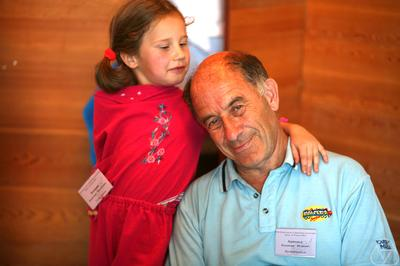
\includegraphics[width=\linewidth]{photo-arnold_small}
}
\date{}

\begin{document}
\maketitle
\thispagestyle{empty}
\cleardoublepage 
\setcounter{page}{1}
\begin{abstract}
\todo{check translation of abstract title}{}Tài liệu này bao gồm 77 bài toán nhằm phát triển văn hóa tư duy, hoặc là được sưu tập, hoặc là được sáng tác bởi tác giả. Hầu hết những bài toán này không yêu cầu bất kỳ một kiến thức đặc biệt nào vượt quá chương trình giáo dục đại cương. Tuy nhiên, việc giải một số bài toán trong số đó có thể thách thức với cả những giáo sư.

	Cuốn sách này được dành cho học sinh, sinh viên đại học, giáo viên và phụ huynh; cho tất cả những ai nghĩ rằng văn hóa tư duy là một phần thiết yếu của sự phát triển nhân cách.
\end{abstract}
\clearpage

\section*{Lời tựa}
Tôi đưa những bài toán này vào tài liệu ở Paris vào mùa xuân năm 2004 khi những người Paris gốc Nga đã nhờ tôi giúp con của họ tăng thêm văn hóa tư duy vốn là truyền thống đối với nước Nga.

Tôi tin chắc rằng văn hóa này hầu như được trau dồi bởi sự tư duy độc lập từ sớm về những điều đơn giản nhưng không phải là những câu hỏi dễ, tương tự như những câu hỏi bên dưới (nhất là các bài toán 1, 3, 13).

Kinh nghiệm của tôi chứng tỏ rằng, thường thường, những người tối dạ trong lớp lại giải các bài toán này tốt hơn những học sinh đạt điểm A, bởi vì -- để trụ lại lớp của họ -- họ phải thường xuyên tư duy nhiều hơn so với những gì được yêu cầu \enquote{để cai quản toàn bộ Seville và Granada}, như Figaro đã dùng để nói về chính ông, trong khi người đạt điểm A không thể nắm bắt được \enquote{cái gì nên nhân với cái gì} trong những bài toán này.

Tôi cũng chú ý rằng những đứa trẻ 5 tuổi giải những bài toán kiểu như vậy tốt hơn những học sinh được rèn luyện, và đến lượt những học sinh này phải đối đầu với những câu hỏi đó, thì họ giải tốt hơn những sinh viên đại học chăm chỉ và những sinh viên này luôn thắng được thầy của họ (những người tệ nhất trong việc giải các bài toán đơn giản này là những người đoạt giải thưởng Nobel và giải thưởng Fields).

\clearpage
\section*{Một số chú ý cho bản dịch tiếng Việt}
Tài liệu \enquote{Các bài toán cho trẻ từ 5 đến 15 tuổi } này được dịch kết hợp từ bản dịch tiếng Anh \enquote{Problems for children from 5 to 15} và bản dịch tiếng Đức \enquote{Denkaufgaben f\"{u}r Kinder von 5-15 Jahren} của cuốn sách nổi tiếng của Vladimir Igorevich Arnold {\selectlanguage{russian}\enquote{{В. И. Арнольд: Задачи для детей от 5 до 15 лет}}}.

Trong bản dịch tiếng Đức, các tác giả đã đưa thêm bảng chú giải một số thuật ngữ liên quan đến các bài toán được đề cập trong tài liệu, và chúng tôi cũng trình bày bản dịch của bảng chú giải này.

Mặc dù đã hết sức cố gắng, nhưng bản dịch tiếng Việt sẽ khó tránh khỏi những thiếu sót. Chúng tôi rất mong nhận được nhiều ý kiến đóng góp của các bạn học sinh, sinh viên, của quý phụ huynh, của các đồng nghiệp nhằm giúp cho bản dịch được hoàn thiện hơn. Mọi ý kiến đóng góp xin gửi đến email \href{mailto:lecongtrinh@qnu.edu.vn}{\nolinkurl{lecongtrinh@qnu.edu.vn}} hoặc \href{mailto:ngolamxuanchau@qnu.edu.vn}{\nolinkurl{ngolamxuanchau@qnu.edu.vn}}. 

\clearpage
\section*{Các bài toán}

\begin{problem}{1.}
	Masha muốn mua một cuốn sách để đọc, nhưng lại thiếu bảy côpêch. Misha cũng muốn mua cuốn sách đó nhưng lại thiếu một côpêch. Thậm chí khi họ muốn góp tiền lại để mua cuốn sách này để đọc chung thì họ cũng không đủ tiền để mua. Hỏi giá của cuốn sách là bao nhiêu?
\end{problem}

\begin{problem}{2.}
	Giá của một cái chai cùng với nút chai là 10 côpêch, trong khi giá của chỉ mình cái chai nhiều hơn giá của cái nút chai là 9 côpêch. Hỏi giá của cái chai không có nút là bao nhiêu?
\end{problem}

\begin{problem}{3.}
	Một viên gạch nặng 1 pao cộng với một nửa cân nặng của viên gạch đó. Hỏi viên gạch này nặng bao nhiêu pao?
\end{problem}

\begin{problem}{4.}
	Rót một thìa rượu từ một thùng rượu vang vào một cốc trà (chưa đầy). Sau đó, rót trở lại vào thùng rượu vang một thìa gồm hỗn hợp rượu và trà được lấy từ cốc trà. Bây giờ trong thùng rượu và trong cốc trà có một thể tích nhất định của chất lỏng từ bên ngoài (rượu vang trong cốc và trà trong thùng). Hỏi thể tích của chất lỏng từ bên ngoài trong cốc trà hay trong thùng rượu vang lớn hơn?
\end{problem}

\begin{problem}{5.}
	Vào lúc mặt trời mọc hai bà già cùng khởi hành (trên cùng một đường), một từ $A$ đến $B$ và một từ $B$ đến $A$. Đến trưa, hai bà gặp nhau, nhưng không dừng lại mà tiếp tục đi với cùng vận tốc như ban đầu của mình. Bà đầu tiên đến $B$ lúc 16 giờ, bà còn lại đến $A$ lúc 21 giờ. Hỏi vào ngày này mặt trời mọc lúc mấy giờ?
\end{problem}

\begin{problem}{6.}
	Trong một bài kiểm tra tiêu chuẩn của Mỹ có câu hỏi sau đây: \enquote{Cho một tam giác vuông có độ dài cạnh huyền bằng 10~insơ, độ dài chiều cao tương ứng với cạnh huyền bằng 6~insơ. Tìm diện tích của tam giác}.

	Hơn một thập kỷ, học sinh trung học Mỹ đã giải bài toán này không khó khăn gì. Nhưng sau đó hỏi câu hỏi trên đối với học sinh trung học Nga đến từ Moskva, không ai có thể giải được như các đồng nghiệp người Mỹ của họ (với đáp số là 30~insơ vuông). Giải thích tại sao?
\end{problem}

\begin{problem}{7.}
	Số chị em gái của Vasya nhiều hơn số anh em trai của anh ta là 2 người. Hỏi rằng số con gái của bố mẹ Vasya nhiều hơn số con trai của họ là bao nhiêu?
\end{problem}

\begin{problem}{8.}
	Cứ vào ngày 01 tháng 06 hàng năm, ở giữa một cái ao tròn ở Nam Mỹ xuất hiện một đóa hoa Victoria Regia. Thân hoa mọc từ dưới đáy ao lên, còn các cánh hoa thì nằm trên mặt nước giống như của hoa súng. Mỗi ngày diện tích của đóa hoa tăng gấp đôi, và cuối cùng vào ngày 01 tháng 07, nó phủ cả mặt hồ, các cánh hoa rơi ra, còn hạt thì chìm xuống đáy. Hỏi vào ngày nào thì diện tích của đóa hoa chiếm một nửa diện tích của ao?
\end{problem}

\begin{problem}{9.}
	Một người nông dân phải đưa một con sói, một con dê và một bắp cải qua sông bằng một chiếc thuyền. Tuy nhiên thuyền của anh ta quá nhỏ, do đó, mỗi lần qua sông anh chỉ mang được mỗi một trong ba đồ vật trên đi cùng với anh ta. Hỏi làm thế nào anh nông dân có thể mang tất cả ba đồ vật trên qua sông, biết rằng con sói không thể để lại ở một mình với con dê, còn con dê thì không thể để ở lại một mình với bắp cải.
\end{problem}

\begin{problem}{10.}
	Một con ốc sên bò lên trên một cái cột cao \SI{10}{\metre}, trên đỉnh có một món mồi ngon (cho ốc sên). Ban ngày nó bò lên được \SI{3}{\cm}, nhưng vào ban đêm, do ngủ nên nó bị tụt xuống \SI{3}{\cm}. Hỏi sau mấy ngày con ốc sên có thể thưởng thức được món mồi ngon?
\end{problem}

\begin{problem}{11.}
	Một nhân viên kiểm lâm từ lều của mình đi bộ về phía nam \SI{10}{\km}, rẽ sang hướng đông và đi tiếp \SI{10}{\km} về hướng đông, gặp anh bạn gấu của anh ta, rẽ sang hướng bắc và đi tiếp \SI{10}{\km} nữa thì về lại lều. Hỏi con gấu màu gì, và nơi đã diễn ra tất cả các sự việc này?
\end{problem}

\begin{problem}{12.}
	Ở một nơi nọ, hôm nay thủy triều dâng lên lúc 12 giờ trưa. Hỏi ngày mai ở nơi này thủy triều sẽ dâng lên vào lúc mấy giờ?
\end{problem}

\begin{problem}{13.}
	Hai tập thơ đầu tiên của Pushkin nằm cạnh nhau trên một kệ sách. Mỗi tập thơ có phần ruột dày \SI{2}{\cm}, còn phần bìa (gồm bìa trước và bìa sau) dày \SI{2}{\mm}. Một con mọt sách gặm (vuông góc với các trang thơ) từ trang đầu tiên của tập một cho đến trang cuối cùng của tập hai. Hỏi đường đi của con mọt sách dài bao nhiêu?

	[Với một đáp án đầy bất ngờ, \SI{4}{\mm}, bài toán tôpô này là nan giải đối với nhiều học giả. Tuy nhiên, một số học sinh mẫu giáo có thể giải bài toán này một cách dễ dàng.]
\end{problem}

\begin{problem}{14.}
	Tìm một vật thể với quan sát từ bên trên xuống và từ phía trước mặt được mô tả như ở hai hình dưới đây (các đa diện). Hãy mô tả các mặt của vật thể (biểu diễn các cạnh ẩn của hình đa diện bằng các nét đứt).
	\begin{figure}
		\footnotesize
		\null\hfill
		\parbox{0.2\linewidth}{\centering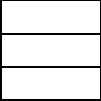
\includegraphics{taskbook-99}\\Nhìn từ bên trên xuống}
		\hfill
		\parbox{0.2\linewidth}{\centering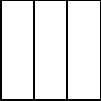
\includegraphics{taskbook-98}\\Nhìn từ phía trước mặt }
		\hfill\null
	\end{figure}
\end{problem}

\begin{problem}{15.}
	Có bao nhiêu cách để phân tích số 64 thành tổng của 10 số tự nhiên, mỗi số trong khoảng từ 1 đến 12? [Hai cách phân tích chỉ khác nhau thứ tự của các hạng tử được xem là như nhau.]
\end{problem}

\begin{problem}{16.}
	Bằng cách đặt một vài thanh giống nhau (chẳng hạn như các quân đôminô), thanh này đặt trên thanh kia, ta nhận được một phần nhô ra với độ dài $x$. Hỏi giá trị lớn nhất có thể đạt được của độ dài của phần nhô ra này?
	\begin{figure}
		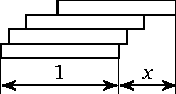
\includegraphics{taskbook-97}
	\end{figure}
\end{problem}

\begin{problem}{17.}
	Hai thành phố $A$ và $B$ cách nhau \SI{40}{\km}. Hai người đi xe đạp xuất phát cùng một lúc theo hai hướng khác nhau, một người xuất phát từ $A$ với vận tốc \SI{10}{\km\per\hour}, người còn lại xuất phát từ $B$ với vận tốc \SI{15}{\km\per\hour}. Một con ruồi bay từ $A$ cùng với người thứ nhất với vận tốc \SI{100}{\km\per\hour}, gặp và chạm vào trán của người thứ hai, sau đó bay ngược lại gặp và chạm vào trán của người thứ nhất, tiếp tục bay ngược lại gặp và chạm vào trán của người thứ hai, và cứ tiếp tục như thế cho đến khi trán của hai người đi xe đạp chạm nhau và đè bẹp con ruồi. Hỏi tổng thể con ruồi đã bay hết bao nhiêu kilômét?
	\begin{figure}
		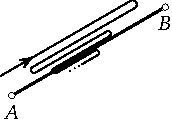
\includegraphics{taskbook-1}
	\end{figure}
\end{problem}

\begin{problem}{18.}
	Biết rằng một quân đôminô che được hai ô vuông trên một bàn cờ. Hãy che cả bàn cờ, trừ hai ô vuông đối diện trên cùng một đường chéo, bằng 31 quân đôminô. [Một bàn cờ có $8\times 8 = 64$ ô vuông.]
	\begin{figure}
		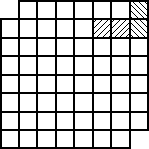
\includegraphics{taskbook-2}
	\end{figure}
\end{problem}

\begin{problem}{19.}
	Một con sâu bướm muốn bò từ một góc của một căn phòng hình lập phương (bên trái trên sàn) đến góc đối diện của căn phòng đó (bên phải trên trần). Tìm đường di chuyển ngắn nhất cho con sâu bướm dọc theo tường của căn phòng.

	\begin{figure}
		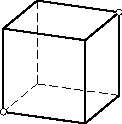
\includegraphics{taskbook-3}
	\end{figure}
\end{problem}

\begin{problem}{20.}
	Bạn có hai cái can, một cái thể tích 5~lít, cái còn lại 3~lít. Làm sao để bạn có thể đo được 1 lít từ hai cái can trên?
	\begin{figure}
		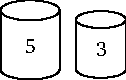
\includegraphics{taskbook-4}
	\end{figure}
\end{problem}
%đầu tiên rót đầy can 5 lít, rót đầy can 3 lít, trong can I còn lại 2 lít. Đổ hết nước can II ra ngoài, đổ 2 lít bên can I vào can II. Đổ đầy vào can I 5 lít, sau đó rót đầy vào can II (đã có 2 lít, chỉ cần rót thêm 1 lít), can I còn lại 4 lít. Đổ nước ở can II ra, rót từ can I vào đầy can II, can I giờ còn 1 lít.

\begin{problem}{21.}
	Trong một gia đình, cả người và chó gồm có 5 cái đầu và 14 cái chân. Hỏi gia đình đó có bao nhiêu người và bao nhiêu con chó?
\end{problem}
%3 người, 2 chó

\begin{problem}{22.}
	Các tam giác đều được dựng bên ngoài trên các cạnh $AB$, $BC$ và $CA$ của tam giác $ABC$. Chứng minh rằng các tâm ($*$) của các tam giác đều này tạo thành một tam giác đều.
	\begin{figure}
		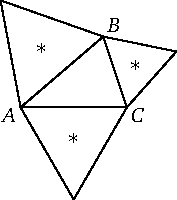
\includegraphics{taskbook-6}
	\end{figure}
\end{problem}

\begin{problem}{23.}
	Nếu cắt một khối lập phương bởi một mặt phẳng, những đa giác có thể nhận được là gì? Chúng ta có thể nhận được một ngũ giác, một thất giác, hay một lục giác đều không?
	\begin{figure}
		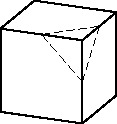
\includegraphics{taskbook-7}
	\end{figure}
\end{problem}

\begin{problem}{24.}
	Hãy vẽ một đường thẳng qua tâm của một khối lập phương sao cho tổng bình phương của các khoảng cách từ tám đỉnh của khối lập phương đến đường thẳng này là a) lớn nhất, b) nhỏ nhất (so với các đường thẳng khác cùng được vẽ qua tâm).
\end{problem}

\begin{problem}{25.}
	Cắt một hình nón tròn thẳng bằng một mặt phẳng dọc theo một đường cong khép kín. Hai quả cầu nội tiếp trong hình nón và tiếp xúc với mặt phẳng lần lượt tại hai điểm $A$ và $B$. Tìm một điểm $C$ trên đường cong bị cắt ở trên để cho tổng các khoảng cách $CA + CB$ là a) lớn nhất, b) nhỏ nhất.
	\begin{figure}
		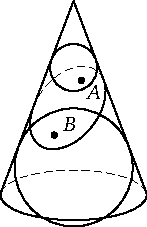
\includegraphics{taskbook-9}
	\end{figure}
\end{problem}

\begin{problem}{26.}
	Một mặt trụ được tạo thành bởi các tiếp tuyến với các đường kinh tuyến của trái đất tại các điểm trên xích đạo. Bề mặt trái đất được chiếu lên mặt trụ này theo các tia song song với xích đạo và cắt trục cực của trái đất. Hỏi rằng diện tích phần được chiếu lên mặt trụ của nước Pháp lớn hơn hay nhỏ hơn diện tích thực của nó?
	\begin{figure}
		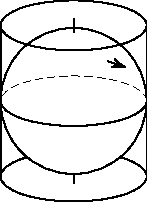
\includegraphics{taskbook-10}
	\end{figure}
\end{problem}

\begin{problem}{27.}
	Chứng minh rằng số dư của phép chia số $2^{p-1}$ cho số nguyên tố lẻ $p$ là $1$ (chẳng hạn, $2^2 = 3a + 1$, $2^4 = 5b+1$, $2^6 = 7c+1$, $2^{10} - 1 = 1023 = 11\cdot 93$).
\end{problem}

\begin{problem}{28.}
	Một cây kim dài \SI{10}{\cm} được ném một cách ngẫu nhiên lên một tờ giấy được kẻ đường với khoảng cách giữa các đường là \SI{10}{\cm}. Điều này được lặp lại $N$ (chẳng hạn, một triệu) lần. Hỏi rằng cây kim giao với một đường trên tờ giấy khoảng bao nhiêu lần (có thể chênh lệch vài phần trăm)?
	\begin{figure}
		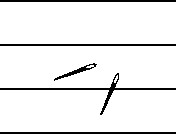
\includegraphics[scale=1]{taskbook-12}
	\end{figure}
	Bạn có thể thực hiện thí nghiệm này với $N=100$ (như tôi đã làm lúc $10$ tuổi) thay vì phải làm một triệu lần. [Đáp số cho câu hỏi này thật ngạc nhiên: $\frac2{\pi}N$. Hơn nữa, thậm chí với một cây kim cong có độ dài $a\cdot \SI{10}{\cm}$, số lần giao nhau quan sát được trên $N$ lần ném sẽ xấp xỉ khoảng $\frac{2a}{\pi}N$. Số $\pi\approx \frac{355}{113}\approx \frac{22}7$.]
\end{problem}

\begin{problem}{29.}
	Các khối đa diện có các mặt bằng nhau được gọi là các \emph{khối Plato}. Chẳng hạn, các khối đa diện với các mặt là tam giác sau đây là các khối Plato: khối tứ diện (4 mặt), khối bát diện (8 mặt), khối nhị thập diện (20 mặt; thật thú vị khi vẽ nó ra, nó có 12 đỉnh và 30 cạnh).\todo{translation of tetra and octa in the figure}{}
	\begin{figure}
		\footnotesize
		\null\hfill
		\parbox{0.3\linewidth}{\centering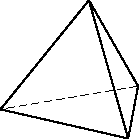
\includegraphics{taskbook-131}\\Khối tứ diện ($\text{tetra}= 4$)}
		\hfill
		\parbox{0.3\linewidth}{\centering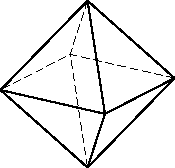
\includegraphics{taskbook-132}\\Khối bát diện ($\text{octo}= 8$)}
		\hfill\null\\
		{\Huge ?}\\Khối nhị thập diện
	\end{figure}
	Kiểm tra xem khẳng định sau đúng hay không: Số mặt của một khối đa diện lồi bị chặn với các mặt là tam giác bằng hai lần số đỉnh trừ đi $4$.

	Thêm một khối Plato sau đây (có tất cả $5$ khối Plato):
	\begin{figure}
		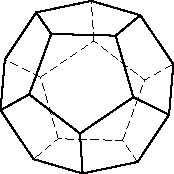
\includegraphics{taskbook-14}
	\end{figure}
\end{problem}

\begin{problem}{30.}
	Một khối mười hai mặt là một khối đa diện lồi với 12 mặt ngũ giác (đều), 20 đỉnh và 30 cạnh (mỗi đỉnh của nó là tâm của một mặt của một khối hai mươi mặt). Hãy vẽ nội tiếp trong một khối mười hai mặt năm khối lập phương (mỗi đỉnh của mỗi khối lập phương là một đỉnh của khối hai mươi mặt) sao cho mỗi cạnh của mỗi khối lập phương là một đường chéo của một mặt nào đó của khối hai mươi mặt (nhớ rằng mỗi khối lập phương có 12 cạnh, mỗi cạnh trên một mặt của khối hai mươi mặt). [Câu hỏi này do Johannes Kepler đưa ra, nhằm mục đích mô tả quỹ đạo của các hành tinh.]
\end{problem}

\begin{problem}{31.}
	Tìm phần giao của hai tứ diện nội tiếp trong một hình lập phương với các tính chất sau đây: mỗi đỉnh của mỗi tứ diện là một đỉnh của khối lập phương, và mỗi cạnh của mỗi tứ diện là một đường chéo của một mặt nào đó của khối lập phương.
	Phần khối lập phương bị chứa trong phần giao của hai khối tứ diện chiếm thể tích là bao nhiêu?
\end{problem}

\begin{problem}{31\textsuperscript{bis}.}
	Hãy dựng giao tuyến của một khối lập phương với một mặt phẳng đi qua ba điểm cho trước trên ba cạnh của khối lập phương đó. [Hãy vẽ đa giác mà qua đó phần mặt phẳng giao với khối lập phương.]
	\begin{figure}
		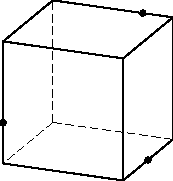
\includegraphics{taskbook-15}
	\end{figure}
\end{problem}

\begin{problem}{32.}
	Một phép đối xứng là một phép biến hình bảo toàn độ dài. Hỏi rằng một khối tứ diện có bao nhiêu phép đối xứng? Một khối lập phương thì có bao nhiêu? khối tám mặt? khối hai mươi mặt? khối mười hai mặt? Trong số đó có bao nhiêu phép quay và bao nhiêu phép phản xạ (đối với một trong năm trường hợp được liệt kê ở trên)?
\end{problem}

\begin{problem}{33.}
	Có bao nhiêu cách để tô màu cho 6 mặt của các khối lập phương giống nhau bằng sáu màu khác nhau $(1,\dotsc,6)$ [mỗi mặt một màu] sao cho không có hai khối lập phương nào được tô màu giống nhau (tức là không có phép quay nào biến khối này thành khối kia)?
	\begin{figure}
		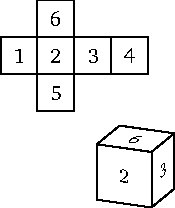
\includegraphics{taskbook-17}
	\end{figure}
\end{problem}

\begin{problem}{34.}
	Có bao nhiêu cách khác nhau để hoán vị $n$ đối tượng?\\
	Có tất cả là sáu cách với $n=3$: $(1,2,3)$, $(1,3,2)$, $(2,1,3)$, $(2,3,1)$, $(3,1,2)$, $(3,2,1)$. Có bao nhiêu cách nếu số đối tượng là $n=4$? $n=5$? $n=6$? $n=10$?
	\begin{figure}
		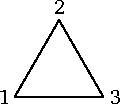
\includegraphics{taskbook-18}
	\end{figure}
\end{problem}

\begin{problem}{35.}
	Một khối lập phương có $4$ đường chéo dài. Hỏi ta có thể nhận được bao nhiêu phép hoán vị khác nhau trên $4$ đường chéo này khi thực hiện các phép quay đối với khối lập phương?
	\begin{figure}
		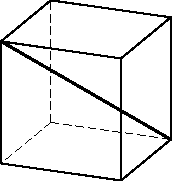
\includegraphics{taskbook-19}
	\end{figure}
\end{problem}

\begin{problem}{36.}
	Hiệu số giữa tổng lập phương của ba số nguyên với lập phương của tổng ba số nguyên đó có luôn chia hết cho $3$ không?
\end{problem}

\begin{problem}{37.}
	Cùng câu hỏi như trên, nhưng với lũy thừa năm và chia hết cho $5$, và với lũy thừa bảy và chi hết cho $7$.
\end{problem}

\begin{problem}{38.}
	Tính tổng
	\begin{equation*}
		\frac{1}{1\cdot 2} + \frac{1}{2\cdot 3} + \frac{1}{3\cdot 4} + \dotsb + \frac{1}{99\cdot 100}
	\end{equation*}
	(với sai số không quá $1\%$ so với đáp số).
\end{problem}

\begin{problem}{39.}
	Chứng minh rằng nếu hai đa giác có diện tích bằng nhau thì ta có thể cắt chúng thành hữu hạn mảnh đa giác nhỏ hơn để khi sắp xếp lại các mảnh này ta sẽ nhận được hai đa giác ban đầu. [Với các vật thể trong không gian, điều này không đúng: khối lập phương và khối tứ diện có thể tích bằng nhau không thể cắt được theo cách này.]
	\begin{figure}
		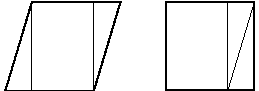
\includegraphics{q39_horizontal}
	\end{figure}
\end{problem}

\begin{problem}{40.}
	Bốn đỉnh của một hình bình hành được đặt tại các nút của một mảnh giấy được kẻ ô vuông sao cho không còn nút nào khác nằm trên cạnh và phần trong của hình bình hành. Chứng minh rằng diện tích của hình bình hành ở trên bằng với diện tích của một ô vuông trên mảnh giấy.
	\begin{figure}
		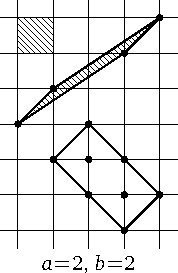
\includegraphics{taskbook-24}
	\end{figure}
\end{problem}

\begin{problem}{41.}
	Dưới các điều kiện của bài toán 40, nếu có $a$ nút chứa trong phần trong và $b$ nút nằm trên các cạnh của hình bình hành thì diện tích của hình bình hành bằng bao nhiêu?
\end{problem}

\begin{problem}{42.}
	Phát biểu tương tự như ở bài toán 40 có còn đúng cho một hình hộp trong không gian 3 chiều hay không?
\end{problem}


\begin{problem}{43.}
	Các số thỏ (hay số Fibonacci) tạo thành một dãy số $(a_1=1)$, $1,2,3,5,8,13,21,34,\dotsc$, trong đó $a_{n+2}=a_{n+1}+a_n$ với bất kỳ $n=1,2,\dotsc$. Tìm ước chung lớn nhất của hai số $a_{100}$ và $a_{99}$.
\end{problem}

\begin{problem}{44.}
	Tìm số (Catalan) tất cả các cách để cắt một $n$-giác lồi thành các tam giác bằng cách cắt dọc theo các đường chéo không giao nhau của nó. Chẳng hạn, $c(4)=2$, $c(5)=5$, $c(6)=14$. Làm thế nào để ta có thể tìm $c(10)$?
	\begin{figure}
		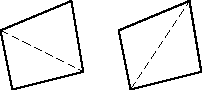
\includegraphics{taskbook-281}
		\qquad
		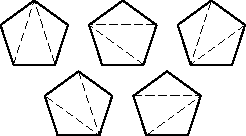
\includegraphics{taskbook-282}
	\end{figure}
\end{problem}

\begin{problem}{45.}
	Một giải đấu cúp có $n$ đội tham gia, mỗi đội thua sẽ rời đi, và đội thắng chung cuộc sẽ được quyết định sau $n-1$ trận đấu. Lịch thi đấu được viết một cách ký hiệu, chẳng hạn như sau, $(a,(b,c),d)$\todo{different example in en\_GB and de\_DE}{} có nghĩa là đội $b$ đấu với đội $c$, đội thắng sẽ gặp đội $a$, và đội thắng trong trận đấu này sẽ gặp đội $d$. Hỏi số lịch thi đấu khác nhau cho một giải đấu gồm $10$ đội tham gia là bao nhiêu?

	\begin{itemize}
		\item Với $2$ đội, ta chỉ có $(a,b)$, và con số này là $1$.
		\item Với $3$ đội, chỉ có $((a,b),c)$, hoặc $ ((a,c),b)$, hoặc $ ((b,c),a)$. Do đó con số này là $3$.
		\item Với $4$ đội, ta có các lịch thi đấu sau đây:
			\begin{equation*}
				\begin{array}{@{}cccc@{}}
					(((a,b),c),d) & \quad\;(((a,c),b),d) & \quad\;(((a,d),b),c) & \quad\;(((b,c),a),d) \\
					(((b,d),a),c) & \quad\;(((c,d),a),b) & \quad\;(((a,b),d),c) & \quad\;(((a,c),d),b) \\ 
					(((a,d),c),b) & \quad\;(((b,c),d),a) & \quad\;(((b,d),c),a) & \quad\;(((c,d),b),a) \\
					((a,b),(c,d)) & \quad\;((a,c),(b,d)) & \quad\;((a,d),(b,c))
				\end{array}
			\end{equation*}
	\end{itemize}
\end{problem}

\begin{problem}{46.}
	Nối $n$ điểm $1, 2, \dotsc, n$ bởi $n-1$ đoạn thẳng để được một cây. Hỏi rằng ta có thể nhận được bao nhiêu cây khác nhau (trường hợp $n=5$ đã thú vị rồi)?

	$n=2$:\quad 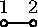
\includegraphics{taskbook-291}\,,\quad số cây nhận được là 1;

	$n=3$:\quad
	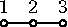
\includegraphics{taskbook-292}\,,\quad
	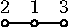
\includegraphics{taskbook-293}\,,\quad
	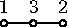
\includegraphics{taskbook-294}\,,\quad
	số cây nhận được là 3;

	$n=4$:\quad\def\quad{\hskip.7em}
	$\vcenter{\hbox{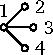
\includegraphics{taskbook-295}}}$,\quad
	$\vcenter{\hbox{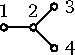
\includegraphics{taskbook-296}}}$,\quad
	$\vcenter{\hbox{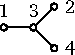
\includegraphics{taskbook-297}}}$,\quad
	$\vcenter{\hbox{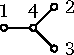
\includegraphics{taskbook-298}}}$,\quad
	$\vcenter{\hbox{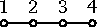
\includegraphics{taskbook-299}}\hbox{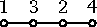
\includegraphics{taskbook-290}}
	\vskip-8pt
	\hbox to50bp{\dotfill}}$,\\
	\null\hspace{\parindent}\phantom{$n=4$:}\quad số cây nhận được là 16.
\end{problem}

\begin{problem}{47.}
	Một phép hoán vị $(x_1, x_2, \dotsc,x_n)$ của các số $\{1, 2, \dotsc,n\}$ được gọi là một \emph{con rắn} (có độ dài $n$) nếu $x_1<x_2>x_3<x_4 \dotsb$.

	\begin{note}{Ví dụ:}\todo{Small caps font}{}
		\begin{equation*}
			\begin{aligned}[t]
				&\begin{aligned}[t] n=2, \text{\ \ ta chỉ có\ \ } 1<2, \end{aligned} &&\text{số con rắn là }1, \\
				&\hskip-\nulldelimiterspace\mathord{\left.\begin{aligned} n=3, \hphantom{\text{\ \ ta chỉ có\ \ }} 1&<3>2 \\ 
				2&<3>1\end{aligned} \right\}}, && \text{số con rắn là }2, \\
				&\hskip-\nulldelimiterspace\mathord{\left.\begin{aligned} n=4, \hphantom{\text{\ \ ta chỉ có\ \ }} 1&<3>2<4 \\ 
				1&<4>2<3 \\ 
				2&<3>1<4 \\ 
				2&<4>1<3 \\ 
				3&<4>1<2\end{aligned} \right\}},
				&&\text{số con rắn là }5. \\
			\end{aligned}
		\end{equation*}
	\end{note}
	Tìm số con rắn có độ dài $10$.
\end{problem}

\begin{problem}{48.}
	Ký hiệu $s_n$ là số con rắn có độ dài $n$:
	\begin{equation*}
		s_1=1, \quad s_2=1, \quad s_3=2, \quad s_4=5, \quad s_5=16, \quad s_6=61.
	\end{equation*}
	Chứng minh rằng chuỗi Taylor của hàm $\tan$ là
	\begin{equation*}
		\tan x=1\, \frac{x^1}{1!}+2\, \frac{x^3}{3!}+16\, \frac{x^5}{5!}+\dots=
		\textstyle\sum\limits_{k=1}^{\infty} s_{2k-1}\, \frac{x^{2k-1}}{(2k-1)!}.
	\end{equation*}
\end{problem}

\begin{problem}{49.}
	Tìm tổng của chuỗi
	\begin{equation*}
		1+1\, \frac{x^2}{2!}+5\, \frac{x^4}{4!}+61\, \frac{x^6}{6!}+\dots=
		\textstyle\sum\limits_{k=0}^{\infty} s_{2k}\,\frac{x^{2k}}{(2k)!}.
	\end{equation*}
\end{problem}

\begin{problem}{50.}
	Với $s>1$, chứng minh đồng nhất thức
	\begin{equation*}
		\textstyle\prod\limits_{p=2}^{\infty} \frac{1}{1-\frac{1}{p^s}}=\textstyle\sum\limits_{n=1}^{\infty} \frac{1}{n^s}.
	\end{equation*}
	(tích được lấy trên tất cả các số nguyên tố $p$, còn tổng được lấy trên tất cả các số tự nhiên $n$).
\end{problem}

\begin{problem}{51.}
	Tìm tổng của chuỗi
	\begin{equation*}
		1+ \frac{1}{4}+ \frac{1}{9}+\dots=\textstyle\sum\limits_{n=1}^{\infty} \frac{1}{n^2}.
	\end{equation*}
	[chứng minh rằng tổng này bằng $\nicefrac{\pi^2}{6}$, tức là, xấp xỉ $\nicefrac{3}{2}$].
\end{problem}

\begin{problem}{52.}
	Tìm xác suất của tính bất khả quy của phân số $\nicefrac{p}{q}$ (tính bất khả quy được định nghĩa như sau: trong đĩa $p^2+q^2 \leqslant R^2$, ta đếm số $N(R)$ các vectơ sao cho số nguyên $p$ và $q$ không có ước chung lớn hơn 1, khi đó xác suất của tính bất khả quy là giới hạn của tỉ số $\nicefrac{N(R)}{M(R)}$, trong đó $M(R)$ là số các điểm nguyên trong đĩa $(M\sim \pi R^2)$).
	\begin{figure}
		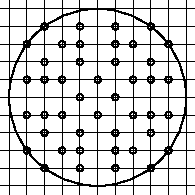
\includegraphics{taskbook-36}\\
		\footnotesize $M(5)=81$, $N(5)=44$, $\nicefrac{N}{M} = \nicefrac{44}{81}$
	\end{figure}
\end{problem}

\begin{problem}{53.}
	Cho $a_n$ là dãy số Fibonacci (xem bài toán 43), hãy tìm giới hạn của tỉ số $\nicefrac{a_{n+1}}{a_n}$ khi $n$ tiến tới vô cùng:
	\begin{equation*}
		\frac{a_{n+1}}{a_n}=2,\ \frac 32,\ \frac53, \ \frac85, \ \frac{13}8,
		\ \frac{34}{21}.
	\end{equation*}
	[Trả lời: Giới hạn đó là \enquote{tỉ số vàng}, $\frac{\sqrt{5}+1}{2}\approx 1,618$. Đây là tỉ số của các cạnh của một hình chữ nhật mà sau khi cắt đi hình vuông có cạnh bằng chiều rộng thì được một hình chữ nhật đồng dạng, $\frac{AB}{BC}=\frac{PC}{CD}$. Tỉ số vàng có liên hệ như thế nào với một ngũ giác đều và với một ngôi sao 5 cánh?]
	\begin{figure}
		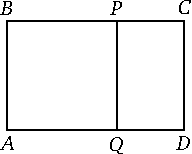
\includegraphics{taskbook-37}
	\end{figure}
\end{problem}

\begin{problem}{54.}
	Hãy tính phân số liên tục vô hạn
	\begin{equation*}
		1+\cfrac{1}{2+\cfrac{1}{1+\cfrac{1}{2+\cfrac{1}{1+\cfrac{1}{2+\ldots}}}}}=
		a_0+\cfrac{1}{a_1+\cfrac{1}{a_2+\cfrac{1}{a_3+\dots}}}
	\end{equation*}
	\todo{add start conditions $a_{2k}=1$ $a_{2k+1}=2$ into the text (cf. en\_GB version)}{}(tức là, tìm giới hạn của phân số 
	\begin{equation*}
		a_0+\cfrac{1}{a_1+\cfrac{1}{a_2+{\atop{\ddots \atop {}} + \cfrac{1}{a_n}}}}
	\end{equation*}
	khi $n\rightarrow \infty)$.
\end{problem}

\begin{problem}{55.}
	Tìm các đa thức 
	\begin{equation*}
		y=\cos 3 (\arccos x),\ y=\cos 4 (\arccos x),\ 
		y=\cos n (\arccos x),
	\end{equation*}
	trong đó $|x| \leqslant 1$.
\end{problem}

\begin{problem}{56.}
	Tính tổng các lũy thừa bậc $k$ của $n$ căn bậc $n$ phức của đơn vị. 
\end{problem}

\begin{problem}{57.}
	Trên mặt phẳng $(x,y)$, hãy vẽ các đường cong có phương trình tham số được cho bởi:
	\begin{equation*}
		\{x=\cos 2t, y=\sin 3t\},\quad 
		\{x=t^3-3t, y=t^4-2t^2\}.
	\end{equation*}
	\vspace{-2\baselineskip}%remove this vertical space if your translation has text coming after the equation
\end{problem}

\begin{problem}{58.}
	Tính (với sai số không quá $10 \%$) $\int_0^{2\pi}\sin^{100}x\,dx$.
\end{problem}

\begin{problem}{59.}
	Tính (với sai số không quá $10 \%$) $\int_1^{10} x^x\,dx$.
\end{problem}

\begin{problem}{60.}
	Tìm diện tích của một tam giác có các góc $(\alpha, \beta, \gamma)$ trên một mặt cầu bán kính 1, biết các cạnh của tam giác là các đường tròn lớn (tức là các giao tuyến của một mặt cầu với các mặt phẳng đi qua tâm của mặt cầu).

	\textbf{Trả lời:}\todo{textbf}{} $S=\alpha+\beta+\gamma -\pi$ (chẳng hạn, đối với một tam giác có ba góc vuông thì $S=\pi/2$, tức là bằng 1/8 tổng diện tích của mặt cầu).
	\begin{figure}
		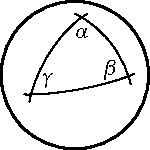
\includegraphics[width=0.2\textwidth]{taskbook-44} \qquad 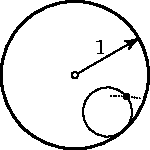
\includegraphics[width=0.2\textwidth]{taskbook-45} 
	\end{figure}
\end{problem}

\begin{problem}{61.}
	Một đường tròn bán kính $r$ lăn (không trượt) bên trong một đường tròn bán kính 1.
	Hãy vẽ toàn bộ quỹ đạo của một điểm thuộc đường tròn lăn (quỹ đạo này được gọi là một hypocycloid) trong trường hợp $r=1/3, r=1/4, r=1/n$, và $r=1/2$. 
\end{problem}

\begin{problem}{62.}
	Trong một lớp $n$ học sinh, hãy ước lượng xác suất để có hai học sinh có cùng ngày sinh nhật. 
	Xác suất đó cao hay thấp?

	\textbf{Trả lời:}\todo{textbf}{} (rất) cao nếu số học sinh là trên (hẳn) $n_0$, (rất) thấp nếu nó dưới (hẳn) $n_0$, và $n_0$ thực chất bằng bao nhiêu để tìm được xác suất $p\approx 1/2$. 
\end{problem}

\begin{problem}{63.}
	Định luật Snell phát biểu rằng góc $\alpha$ tạo bởi một tia sáng với pháp tuyến của các lớp của một môi trường phân tầng thỏa mãn phương trình $n(y) \sin \alpha =\mbox{const}$, trong đó $n(y)$ là chỉ số khúc xạ của tầng ở độ cao $y$ (đại lượng $n$ là tỉ lệ nghịch với vận tốc ánh sáng trong môi trường đó khi lấy vận tốc ánh sáng trong chân không bằng 1; trong nước $n=\dfrac{4}{3}$).

	\begin{figure}
	%\includegraphics[width=0.5\textwidth]{snell-law.jpg}
	\centering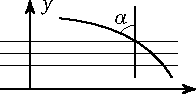
\includegraphics[width=0.3\textwidth]{taskbook-47} 
	\qquad
	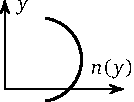
\includegraphics[width=0.2\textwidth]{taskbook-471} 
	\end{figure}
	Hãy vẽ các quỹ đạo của tia sáng trong môi trường \enquote{không khí trên sa mạc}, trong đó chỉ số $n(y)$ đạt cực đại ở một độ cao nào đó (lời giải cho bài toán này cũng giải thích những ảo giác trên sa mạc để ta hiểu quỹ đạo của các tia sáng phát ra từ các đồ vật có liên hệ thế nào với các ảnh).
\end{problem}

\begin{problem}{64.}
	Hãy nội tiếp trong tam giác nhọn $ABC$ một tam giác $KLM$ có chu vi bé nhất (với các đỉnh $K$ trên $AB$, $L$ trên $BC$, $M$ trên $CA$).

	\textsc{Hướng dẫn}:\todo{textsc}{} Với các tam giác không nhọn lời giải không đẹp như với các tam giác nhọn. 
	\begin{figure}
		\centering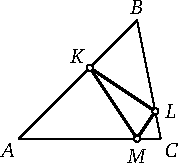
\includegraphics[width=0.2\textwidth]{taskbook-48}
	\end{figure}
\end{problem}

\begin{problem}{65.}
	Tính giá trị trung bình của hàm $1/r$ (trong đó $r^2=x^2+y^2+z^2$, $r$ là khoảng cách tới gốc tọa độ) trên mặt cầu bán kính $R$ có tâm tại điểm $(X,Y,Z)$.

	\textsc{Hướng dẫn}:\todo{textsc}{} Bài toán này liên quan đến định luật vạn vật hấp dẫn của Newton và định luật Cu-lông của lý thuyết điện trường. Đối với trường hợp hai chiều của bài toán thì nên thay hàm đang xét bằng $\ln r$ và thay mặt cầu bằng đường tròn.
\end{problem}

\begin{problem}{66.}
	Từ $2^{10}=1024\approx 10^3$ suy ra $\log_{10}2\approx 0,3$. Hãy ước lượng sai số và tính $\log_{10}2$ tới 3 chữ số thập phân.
\end{problem}

\begin{problem}{67.}
	Với cùng độ chính xác như trên hãy tính $\log_{10}4, \log_{10}8, \log_{10}5,$ $ \log_{10}50, \log_{10}32, \log_{10}128, \log_{10}125, \log_{10}64.$
\end{problem}

\begin{problem}{68.}
	Sử dụng $7^2\approx 50$ để tìm giá trị xấp xỉ của $\log_{10}7$. 
\end{problem}

\begin{problem}{69.}
	Cho biết $\log_{10}64$ và $\log_{10}7$, hãy tìm $\log_{10}9, \log_{10}3, \log_{10}27, \log_{10}6,$ $ \log_{10}12$.
\end{problem}

\begin{problem}{70.}
	Sử dụng $\ln(1+x)\approx x$ ($\ln$ là $\log_e$) để tìm $\log_{10}e$ và $\ln 10$ dựa vào quan hệ\footnote{Số Euler $e=2,71828\ldots$ được xác định bằng giới hạn của dãy $\left(1+\dfrac{1}{n}\right)^n$ khi $n\rightarrow \infty$, và bằng tổng của chuỗi $1+\dfrac{1}{1!}+\dfrac{1}{2!}+\dfrac{1}{3!}+\cdots$. Nó cũng có thể được xác định qua công thức: $\lim\limits_{x\rightarrow 0}\dfrac{\ln(1+x)}{x}=1$.}
	$$\log_{10}a=\dfrac{\ln a}{\ln 10}$$
	và từ các giá trị của $\log_{10}a$ đã tính trước đó (chẳng hạn, với $a=128/125, 1024/1000$ và vân vân).

	[Lời giải cho các bài toán 65-69 đưa ra một bảng các lôgarít 4 chữ số của bất kỳ số nào sử dụng các tích các số đã tìm được như là dữ liệu cơ sở và dùng công thức $$\ln(1+x)\approx x-\dfrac{x^2}{2}+\dfrac{x^3}{3}-\dfrac{x^4}{4}+\cdots$$ cho sự hiệu chỉnh.] (Bằng cách này Newton đã biên soạn được một bảng các logarit 40 chữ số!)
\end{problem}

\begin{problem}{71.}
	Xét dãy các lũy thừa của hai: 1, 2, 4, 8, 16, 32, 64, 128, 256, 512, 1024, 2048, $\ldots$. Trong số 12 số đầu tiên, có 4 số có biểu diễn thập phân bắt đầu bằng chữ số 1 và không có số nào bắt đầu bằng chữ số 7. Chứng minh rằng khi $n\rightarrow \infty$ chữ số đầu tiên của số $2^m$, $0\leq m\leq n$, sẽ lặp lại với một tần số nào đó: 
$p_1\approx 30\%, p_2\approx 18\%, \ldots, p_9 \approx 4\%$.
\end{problem}

\begin{problem}{72.}
	Hãy kiểm tra lại quy luật các chữ số đầu tiên của các lũy thừa của ba: 1, 3, 9, 2, 8, 2, 7, $\ldots$. Chứng minh rằng khi $n\rightarrow \infty$ ta cũng được những tần số nào đó và hơn nữa, tần số đó giống với trường hợp các lũy thừa của hai. Hãy tìm một công thức chính xác cho $p_1,\ldots, p_9$.

	\textsc{Hướng dẫn}:\todo{textsc}{} Chữ số đầu tiên của một số $x$ được xác định bằng phần thập phân của số $\log_{10}x$, do đó ta phải xét dãy các phần thập phân của số $m\alpha$, trong đó $\alpha=\log_{10}2$.

	Chứng minh rằng những phần thập phân này được phân bố đều trên khoảng từ 0 đến 1, tức là: bên ngoài $n$ phần thập phân của số $m\alpha$, $0\leq m<n$, một khoảng con $A$ sẽ chứa đại lượng $k_n(A)$ sao cho, khi $n\rightarrow \infty$, $\lim(k_n(A)/n)=(\mbox{độ dài khoảng con } A)$.
\end{problem}

\begin{problem}{73.}
	Cho $g: M\rightarrow M$ là một ánh xạ trơn từ một miền bị chặn $M$ lên chính nó, sao cho $g$ là 1-1 và bảo toàn diện tích ( là thể tích trong trường hợp nhiều chiều) của miền. Chứng minh rằng trong một lân cận $U$ bất kỳ của một điểm bất kỳ của $M$ và với bất kỳ số nguyên dương $N$, tồn tại một điểm $x$ sao cho $g^Tx$ cũng thuộc $U$ với số nguyên $T>N$ nào đó (\enquote{định lý hồi quy}).
\end{problem}

\begin{problem}{74.}
	Cho $M$ là mặt xuyến (với các tọa độ $\alpha({\rm mod} 2\pi), \beta({\rm mod} 2\pi)$), và $g(\alpha,\beta)=(\alpha+1,\beta+\sqrt{2})({\rm mod} 2\pi)$. Chứng minh rằng dãy điểm $\{g^Tx\}$, $T=1,2,\ldots,$ là trù mật khắp nơi trong xuyến.
	\begin{figure}
		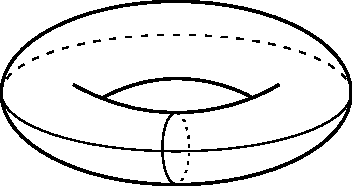
\includegraphics[width=0.2\textwidth]{74_torus}
	\end{figure}
\end{problem}

\begin{problem}{75.}
	Với ký hiệu như ở bài toán 74, cho
	$$g(\alpha, \beta)=(2\alpha+\beta, \alpha+\beta) \; ({\rm mod} 2\pi).$$
	Chứng minh rằng tồn tại một tập con trù mật khắp nơi của xuyến bao gồm các điểm tuần hoàn $x$ (tức là, thỏa mãn $g^{T(x)}x=x$ với số nguyên $T>0$ nào đó).
\end{problem}

\begin{problem}{76.}
	Với ký hiệu như ở bài toán 74 chứng minh rằng với hầu hết tất cả các điểm $x$ của xuyến, dãy điểm $\{g^T(x)\}$, $T=1,2,\ldots,$ là trù mật khắp nơi trong xuyến (các điểm $x$ không có tính chất này tạo thành một tập có độ đo không).
\end{problem}

\begin{problem}{77.}
	Với ký hiệu như ở bài toán 74 và 76 chứng minh rằng dãy $\{g^T(x)\}$, $T=1,2,\ldots,$ được phân phối đều trên xuyến: nếu một miền $A$ chứa $k_n(A)$ điểm trong số $n$ điểm với $T=1,2,\ldots, n$ thì
	$$\lim_{n\rightarrow \infty}\frac{k_n(A)}{n}=\frac{\mbox{mes}(A)}{\mbox{mes}(M)}$$
	(chẳng hạn, với một miền đo được Jordan $A$ có độ đo $\mbox{mes} A$).
\end{problem}

\begin{note}{Chú ý đối với bài toán 13.}
	Tôi đã cố gắng minh họa cho sự khác biệt trong cách tiếp cận công việc của các nhà toán học và các nhà vật lý bằng bài toán này, trong bài báo mời của tôi trên tạp chí \enquote{Physics -- Uspekhi} nhân dịp mừng Giáng sinh năm 2000. Thành công của tôi vượt xa những gì tôi đã dự kiến: không như các em học sinh mẫu giáo, đối tượng nền tảng cho kinh nghiệm của tôi, các biên tập viên bị sai khi giải bài toán này, và do đó họ đã sửa đề bài lại cho đúng với đáp án 4mm của tôi như sau: thay vì \enquote{từ trang đầu tiên của tập một cho đến trang cuối cùng của tập hai} họ sửa lại thành \enquote{từ trang \emph{cuối cùng} của tập một đến trang \emph{đầu tiên} của tập hai}.

	Câu chuyện có thật này kinh ngạc đến mức tôi đề cập nó ở đây: chứng minh là phiên bản của các biên tập viên được đăng trên tạp chí.
\end{note}
\clearpage

\section*{Bảng chú giải thuật ngữ}
\begin{description}
	\item[trù mật] Một tập con $A$ của một tập \enquote{lớn} $M$ được gọi là \emph{trù mật} trong $M$ nếu mỗi phần tử của $M$ có thể xấp xỉ với một dãy các phần trong $A$(tức là, nếu mỗi phần tử trong $M$ \enquote{gần} tùy ý với một phần tử trong $A$).

		Chẳng hạn, tập số các hữu tỷ $\mathbb Q$ trù mật trong tập hợp các số thực $\mathbb R$, tức là, mỗi số thực có thể được xấp xỉ bằng một dãy các phân số. 

	\item[căn của đơn vị] Một \emph{căn bậc $n$ của đơn vị } là một số mà lũy thừa bậc $n$ của nó bằng 1 (viết bằng công thức: là một số $z$ sao cho $z^n=1$). 

		Chẳng hạn $1$ là một căn bậc $n$ của đơn vị đối với mỗi số tự nhiên $n$, bởi vì $1^n=1$. Nếu $n$ là một số chẵn thì $-1$ cũng là một căn bậc $n$ của đơn vị, bởi vì $(-1)^n=1$.

		Trong trường hợp tổng quát, các căn của đơn vị chứa trong trường các số phức. Đây là trường số kế tiếp lớn nhất phía trên tập các số thực. 

	\item[dãy] Một \emph{dãy} là một danh sách gồm các đối tượng được đánh số theo một luật cấu thành nào đó. Mỗi dãy được ký hiệu bởi $(a_n) = a_1,a_2,a_3,\dots $, trong đó $a_n$ được gọi là phần tử thứ $n$ của dãy. 

		Ví dụ:
		\begin{itemize}
		\item Các số tự nhiên với luật cấu thành $a_n = n$:
		\begin{equation*}
		1,2,3,4,5,\dots{}
		\end{equation*}
		Ta có thể trích ra các phần tử riêng lẻ của dãy, chẳng hạn $a_{14} = 14$. 
		\item Các số Fibonacci với luật cấu thành $a_n = a_{n-1}+a_{n-2}$ và với các giá trị ban đầu $a_1 = a_2 = 1$:
		\begin{equation*}
		1,1,2,3,5,8,13,\dots{}
		\end{equation*}
		\item Dãy được tạo ta bởi luật cấu thành $a_n = f^n(x)$ với hàm $f(x) = 2x-1$. Để xác định được dãy này, dĩ nhiên ta cần có một giá trị ban đầu nào đó của $x$, chẳng hạn $x=2$: 
		\begin{equation*}
		a_1 = f(2) = 3,\ a_2 = f(3) = 5,\ a_3 = f(5) = 9,\dots
		\end{equation*}
		Ta cũng có thể viết dãy ở dạng khác như sau: $3,5,9,17,33\dots{}$
		\end{itemize}

	\item[ánh xạ trơn] Theo định nghĩa toán học, một ánh xạ được gọi là \emph{trơn} nếu nó khả vi vô hạn. Chẳng hạn mỗi đa thức là một ánh xạ trơn:
		\begin{gather*}
		f(x) = x^2 + 3,\ f'(x) = 2x,\ f''(x) = 2,\\
		f'''(x) = f^{(n)}(x) = 0 \text{ với mọi số tự nhiên } n.
		\end{gather*}
		Hàm $e$ mũ cũng là một ánh xạ trơn: 
		\begin{equation*}
		g(x) = e^x, g'(x) = g^{(n)}(x) = e^x \text{ với mọi số tự nhiên } n.
		\end{equation*}
		Một ví dụ về một hàm không trơn là hàm giá trị tuyệt đối $h(x) = |x|.$ Nó có một \enquote{đỉnh} tại $x=0$ và nó không khả vi tại đó.

		Rõ ràng thuật ngữ \enquote{trơn} cho các hàm được hiểu theo nghĩa đen: đồ thị của một hàm trơn không có bất kỳ một đỉnh nào.

	\item[đơn ánh] Một ánh xạ được gọi là \emph{đơn ánh} nếu mỗi phần tử trong tập đích có nhiều nhất là một phần tử bên tập nguồn để đặt tương ứng với nó. Chẳng hạn, mỗi phép hoán vị là một đơn ánh. 

		Ví dụ:
		\begin{figure}[H] 
			\centering 
			\def\svgwidth{200pt} 
			\input{glossar_injektiv.pdf_tex} 
		\end{figure}
		Hàm số $f(x) = x^2$ không phải là một đơn ánh nếu miền xác định của nó là tập hợp các số thực $\mathbb R$. Thật vậy, chẳng hạn ta có $f(-1) = f(1) = 1$, do đó có hai phần tử khác nhau là 1 và -1 trong tập nguồn cùng đặt tương ứng với phần tử 1 trong tập đích.

	\item[lồi] Các nhà toán học gọi một hình (chẳng hạn, một đa diện) là \emph{lồi} nếu qua hai điểm bất kỳ của nó ta luôn có thể vẽ được một đoạn thẳng nằm hoàn toàn trong nó. Một cách hình ảnh, một hình lồi cong ra phía ngoài ở khắp mọi nơi.

		Ví dụ: 
		\begin{figure} 
			\def\svgwidth{270pt} 
			\input{glossar_konvex.pdf_tex} 
		\end{figure}

	\item[môđun] Ta viết $a \mod b$ có nghĩa là số dư của phép chia $a$ cho $b$. 

		$c\equiv a \operatorname{mod} b$ (đọc là \enquote{$c$ đồng dư với $a$ theo môđun $b$}) có nghĩa là $c$ và $a$ có cùng số dư khi chia cho $b$. 

		Ví dụ: $7\equiv 1\operatorname{mod} 6,\ 11\equiv 3\operatorname{mod} 4$. 

	\item[phép hoán vị] Một phép hoán vị là một ánh xạ biến các số $1,2,\dots,n$ thành các số $1,2,\dots,n$ sao cho mỗi số đều có mặt trong tập ảnh. 

		Ví dụ:
		\begin{figure} 
			\def\svgwidth{200pt} 
			\input{glossar_permutation.pdf_tex} 
		\end{figure} 
	
	\item[ký hiệu tích] Tương tự như ký hiệu tổng, ký hiệu tích $\prod$ là một cách viết tắt cho cụm từ \enquote{nhân các số này với nhau}. Các cận của tích được viết ở phía dưới và phía trên của ký hiệu tích.

		Ví dụ: 
		\begin{gather*}
			\prod\limits_{k=3}^5 k = 3\cdot 4\cdot 5 = 60,\\
			\prod\limits_{m=4}^7 (m^2 - m) = (4^2-4)\cdot(5^2-5)\cdot (6^2-6) \cdot (7^2-7)= 302\,400.
		\end{gather*}
		\item[ký hiệu tổng] Ký hiệu tổng là một cách viết tắt cho cụm từ \enquote{cộng các số này lại}. Cận dưới (bắt đầu) được viết ở phía bên dưới và cận trên (kết thúc) được viết ở phía bên trên của ký hiệu tổng, cho ta biết được tổng được lấy từ đâu đến đâu:		
		\begin{equation*}
			\sum\limits_{i=1}^5 i,
		\end{equation*}
		được đọc là \enquote{tổng lấy theo $i$ từ 1 đến 5}, có nghĩa là lấy tổng các số từ 1 đến 5. 

		Ví dụ:
		\begin{gather*}
			\sum\limits_{i=7}^{11} i= 7+8+9+10+11 = 45,\\
			\sum\limits_{i=1}^3 i\cdot (i+2) = 1\cdot (1+2) + 2\cdot (2+2) + 3\cdot (3+2) = 26.
		\end{gather*}
		Ta cũng có thể lấy tổng không có cận trên, có nghĩa là cận trên của tổng tiến ra vô hạn. Khi đó ta viết $\sum\limits_{i=1}^\infty$. 
\end{description}

\clearpage
\null\vfill
\noindent
Dịch từ tiếng Nga sang tiếng Anh bởi \\
\null\quad Victor Goryunov và Sabir Gusein-Zade\\
\\
Dịch từ tiếng Anh sang tiếng Đức bởi \\
\null\quad David Gr\"{u}nberg, Lilian Hueber và Lea Renner\\
\\
Dịch từ tiếng Anh và tiếng Đức sang tiếng Việt bởi \\
\null\quad Ngô Lâm Xuân Châu và Lê Công Trình \\
\\
Bản gốc tiếng Nga:\\
\null\quad {\selectlanguage{russian}{В. И. Арнольд: Задачи для детей от 5 до 15 лет}}\\
\null\quad Moscow, MCCME, 2004\\
\null\quad ISBN 5-94057-183-2\\
\\
\\
Ảnh bìa được cung cấp bởi:\\ 
\null\quad Trung tâm lưu trữ của Viện Nghiên cứu Toán học Oberwolfach\\
\\
Cuốn sách này được phát hành theo giấy phép CC BY-NC-SA 3.0 tại diễn đàn IMAGINRAY: \href{http://www.imaginary.org/background-materials}{www.imaginary.org/background-materials}.\\
IMAGINARY là một dự án của Viện Nghiên cứu Toán học Oberwolfach dưới sự tài trợ của quỹ Klaus Tschira.
\end{document}
